\documentclass[../master.tex]{subfiles}
\graphicspath{{\subfix{../figures/test/}}}

\begin{document}

\section{Why Start with Arithmetic?}
Nothing to note here...

\section{Addition}
% 
\includegraphics[scale=0.6]{11} %how to insert an <hr> here?
% 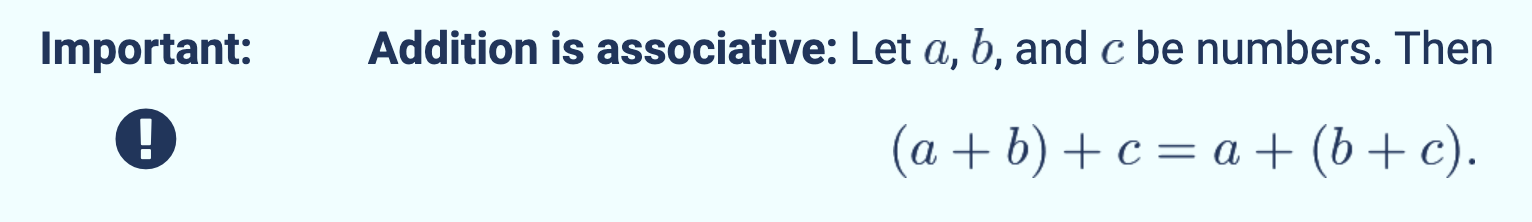
\includegraphics[scale=0.6]{12}
% 
\includegraphics[scale=0.48]{13}
Together, the commutative and associative properties are sneakily powerful, as they let us add a list of numbers in any order. It is also called the  any-order principle.


\section{Negation}
% \includegraphics[scale=0.44]{4}	
% \includegraphics[scale=0.44]{}

\end{document}


